\begin{exercise}
      {ID-ca9744696cf60bcbd003bcff5f9667a7fbef5a8f}
      {Quadrat}
  \ifproblem\problem\par
    \begin{minipage}{0.25\textwidth}
      \centering
      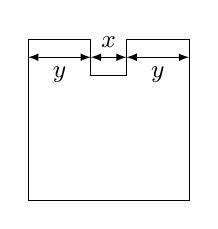
\begin{tikzpicture}[scale=0.75]
        \draw [line width=0.4pt]
              ( 0ex,  0ex) -- (18ex,  0ex) -- (18ex, 18ex) --
              (11ex, 18ex) -- (11ex, 14ex) -- ( 7ex, 14ex) --
              ( 7ex, 18ex) -- ( 0ex, 18ex) -- cycle;
        \draw[line width=0.3pt, <->, >=latex] ( 0ex, 16ex) -- node[below] {{\small$y$}} ( 7ex, 16ex);
        \draw[line width=0.3pt, <->, >=latex] ( 7ex, 16ex) -- node[above] {{\small$x$}} (11ex, 16ex);
        \draw[line width=0.3pt, <->, >=latex] (11ex, 16ex) -- node[below] {{\small$y$}} (18ex, 16ex);
      \end{tikzpicture}
    \end{minipage}\hfill
    \begin{minipage}{0.70\textwidth}
      Aus einem \sicm{80} langen Draht soll eine quadratische Figur mit einer
      quadratischen Aussparung gebogen werden. Gib eine Gleichung für den
      Umfang und eine mögliche Lösung an.
    \end{minipage}
  \fi
  %\ifoutline\outline\par
  %\fi
  %\ifoutcome\outcome\par
  %\fi
\end{exercise}
